%tag:000X
%label:dig:viterboSuggestive
%type:diagram
%author:JeffHicks

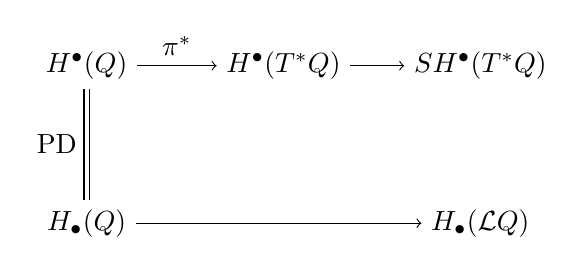
\begin{tikzpicture}

\node (v3) at (-2.5,1.5) {$H^\bullet(Q)$};
\node (v4) at (-2.5,-0.5) {$H_\bullet(Q)$};
\node (v1) at (0,1.5) {$H^\bullet(T^*Q)$};
\node (v5) at (2.5,-0.5) {$H_\bullet(\mathcal L Q)$};
\node (v2) at (2.5,1.5) {$SH^\bullet(T^*Q)$};

\draw  (v1) edge[->]  (v2);
\draw  (v3) edge[->]node[above]{$\pi^*$} (v1);
\draw  (v4) edge[->] (v5);
\draw  (v3) edge[double equal sign distance] node[left]{PD} (v4);
\end{tikzpicture}